\documentclass[11pt, notitlepage]{report}

\usepackage[tmargin=2cm, lmargin=2cm, rmargin=2cm, bmargin=3cm]{geometry}
\usepackage{parskip}
\usepackage[latin1]{inputenc}
\usepackage{graphicx}
\usepackage{wrapfig}
\usepackage{hyperref}

\begin{document}


\title{MAlice Report}
\author{Owen Davies, Daniel Hertz, Charlie Hothersall-Thomas}
\date{\today}

\maketitle

\section*{The Product}
Our compiler is largely successful and generally meets the criteria set out in the specification for the project. In particular, the syntactic and semantic analysis components of the compiler are extremely sound. There are some small bugs in the code generation portion of the compiler, which we would have liked to fix if we had had more time to spend on the project.

We think that it would be fairly easy to further develop our compiler. The use of a class-based system for our AST (with a seperate class for each node) means that it is very easy to add new language features - one can simply add new node classes that extend the \texttt{ASTNode} class, and add methods in the \texttt{TreeWalker} class to create the new node objects. Similarly, in the code generation stage, one can just add new methods to the \texttt{ASTVisitor} class to process the new AST node types. This is one of the benefits of using the visitor pattern to generate code from an AST.

We chose to write our compiler in C++. We made this decision because we wanted to create an object-based solution (to take advantage of design patterns like the visitor pattern), and we also wanted to use this project as an opportunity to further develop our skills in the language - something we feel we have definitely achieved. C++ also has notable performance advantages over other object-oriented languages such as Java. We chose to compile down to ARM Assembly for similar reasons: ARM is an architecture in which we are all interested (and also one that is growing in popularity very quickly), but not one that we knew much about. We therefore saw this as a good opportunity to learn more about it. We also wanted to take advantage of the Raspberry Pi we had available for use in the project, so compiling down to ARM was the obvious option.

Throughout the project we used the \texttt{boost} C++ libraries; in particular \texttt{boost::shared\_ptr} to make memory management simpler (we were initially using raw pointers, but managing these in the semantic analysis stage became very complex). Whilst using \texttt{shared\_ptr}s definitely made the code simpler, they are significantly slower than raw pointers (due to the built-in reference counting). In this case, we decided to sacrifice performance for simplicity.

\section*{Design Choices}
For the lexical and syntactic analysis aspects of the compiler, we decided to use the lexer and parser generator tool \emph{ANTLRv3}. Our success with this tool was mixed due to its steep learning curve, which meant that initial progress was very slow. \emph{ANTLR} was originally written with Java as a language target. We wanted to use C++, and it soon became apparent that the documentation was distinctly lacking for the C++ target. In fact, the \emph{ANTLR} C++ target was so limited that we decided to use the C target instead, which had more features and fair bit more documentation. We could then write C++ code on top of the generated C code.

This approach proved far more successful, and we were soon making rapid progress through the lexing and parsing of the MAlice language. Once one gets to grips with \emph{ANTLR}, it proves to be an incredibly powerful tool. In particular, two features were found to be very useful:
\begin{itemize}
\item \textbf{Syntactic Predicates} - This feature allows you to tell \emph{ANLTR} to look ahead at the next \emph{n} tokens and check to see if the input conforms to this subrule. If it doesn't, \emph{ANTLR} moves to the next rule. This is written as such:
\begin{center}
	\texttt{rule: (A B C) => x | y}
\end{center}
The above rule says ``If \texttt{(A B C)} holds for the current token stream then do \texttt{x}, otherwise do \texttt{y}''. This feature allowed us to get around any ambiguity in the MAlice language very easily.

\item \textbf{Rewrite Rules} - This allows the user to map an input stream to an output tree. This comes in very handy when creating a parse tree, as you can create imaginary nodes for your parse tree that come in very useful when walking the tree later on:
\begin{center}
	\texttt{rule: a b `.' -> \textasciicircum(TOK a b)}
\end{center}
This creates a new sub-tree in the parse tree with \texttt{TOK} as the root node. This rewrite system is also very useful for defining operator precedence, since you can make the binary operator the root node of its own subtree, and the expression automatically has the correct precedence.
\end{itemize}
If we'd have had the opportunity to go back and redo the project, we would have looked at more options for lexer and parser generation in C++, to avoid the inital few days of wrestling with \emph{ANTLR}, trying to get it to behave as we wished. However, it is an excellent tool once you start to understand it properly.

We decided to manually write the semantic analysis component of our compiler. We could have perhaps used \emph{ANTLR} for this section as well, but decided that we didn't have enough time to learn the necessary complex aspects of the tool well enough to create a good solution with them. Additionally, the lectures we had been given on semantic analysis were comprehensive enough such that we felt equipped to hand craft this aspect of the compiler.

As mentioned in the introduction, code generation was implemented using the visitor pattern on our AST nodes. Each \texttt{ASTNode} class has an \texttt{accept} method, which tells its visitor everything it knows about itself after semantic analysis (e.g.\ name, type, enclosing symbol table). The visitor, \texttt{ASTVisitor}, then has a method for each class that extends \texttt{ASTNode}, which calls the relevant accept methods and generates any assembly code required for the program.

\section*{Beyond the Specification}
\subsection*{Optimisations}
We have made a number of optimisations in our compiler:
\begin{itemize}
\item \textbf{Removing unecessary \texttt{mov} instructions and sequences} - any instructions of the form \texttt{mov ri ri} and instruction sequences of the form \texttt{mov ri rx ... mov ry ri} are removed.
\item \textbf{Removing uncalled functions} - any functions with are not called in the program (and hence are dead code) are removed from the program code.
\item \textbf{Removing empty statement blocks} - any \texttt{perhaps}, \texttt{either}, or \texttt{eventually} code blocks without a body are removed. This removal is done before code generation to avoid generating code which will later be removed.
\item \textbf{Register allocation} - before the instructions for an expression are generated, we apply a weighting algorithm to the expression tree which attempts to work out the ``cost'' of each sub-expression, and therefore the most sensible order in which to allocate registers for the expression (we want to generate code for the ``cheapest'' expression first). Expressions like \texttt{(2 * x + y) + x} would normally be evaluated left to right, but it's more efficient to generate code for the right hand side first in this case. We also make sure that two registers never hold the same expression, to try to prevent the program from running out of registers for as long as possible.
\end{itemize}

\subsection*{Extension - Hardware IO in MAlice}
Since we had already decided to compile down to ARM assembly, and had a Raspberry Pi available, we thought that it would be fun to extend MAlice to have commands for hardware IO. This was possible due to the GPIO (general-purpose IO) registers present in an ARM microcontroller such as the Pi. We therefore wrote new MAlice commands to control the GPIO pins on the Raspberry Pi. The following MAlice code shows the new commands included in our extended version of MAlice:

\begin{verbatim}
###include io
The looking-glass hatta()
opened
    x was a number.

    The Caterpillar blew out 4 smoke rings. ### make IO4 an output pin
    The Caterpillar inhaled 24 times.       ### make IO24 an input pin

    The rabbit jumped.                      ### enable pull-up resistors on IO24 and IO25

    Alice discovered x through door 24.     ### x = 0 or 1, depending on IO24's value

    4 said Tweedledee.                      ### set pin IO4 high
    Alice slept for 100 milliseconds.       ### sleep for 100ms
    4 said Tweedledum.                      ### set pin IO4 low
closed
\end{verbatim}

Certain Raspberry PI IO pins have internal pull-up resistors, which can be enabled on request. This means that an input switch can be connected directly from ground, with no need for an external pull-up resistor to 3.3V. The \texttt{The rabbit jumped} command enables these internal pull-up resistors on pins IO24 and IO25.

The implementation of these new commands required changes to almost every element of the compiler. This is where our design choices came into play, as it took minimal effort to add the commands to the language and output their ARM assembly code. The majority of time allocated to the extension was spent getting to grips with the Raspberry Pi's (somewhat undocumented) GPIO controller.

Initially, we hooked our Pi up to a simple LED circuit and used a pre-written Python library to blink the LED. We did this to confirm that the LED was wired up correctly, and were then ready to try hardware IO at a lower level.$  $

We used C's \texttt{mmap} function to map from Linux virtual addresses to the physical hardware address of the Pi's GPIO controller. From here, hardware IO was a case of using integer division/modulo arithmetic and bitwise operations to manipulate the correct pin (pins are stored in blocks of 10, and each pin is represented by 3 bits). For programs that use IO commands, the C file which controls memory mapping and other IO utils is compiled and linked with the program's generated assembly at compile time. This is why \texttt{\#\#\#include io} is required as the first line of the file, to tell the preprocessor to change the assemble command.

\subsection*{Extension Demonstration: `Town Called MAlice'}

At this stage, we had simple MAlice programs blinking LEDs and reading inputs from physical switches, using our new commands. However, we wanted to demonstrate the power of IO-enriched MAlice properly.

\begin{wrapfigure}{r}{0.3\textwidth}
  \vspace{-20pt}
  \begin{center}
    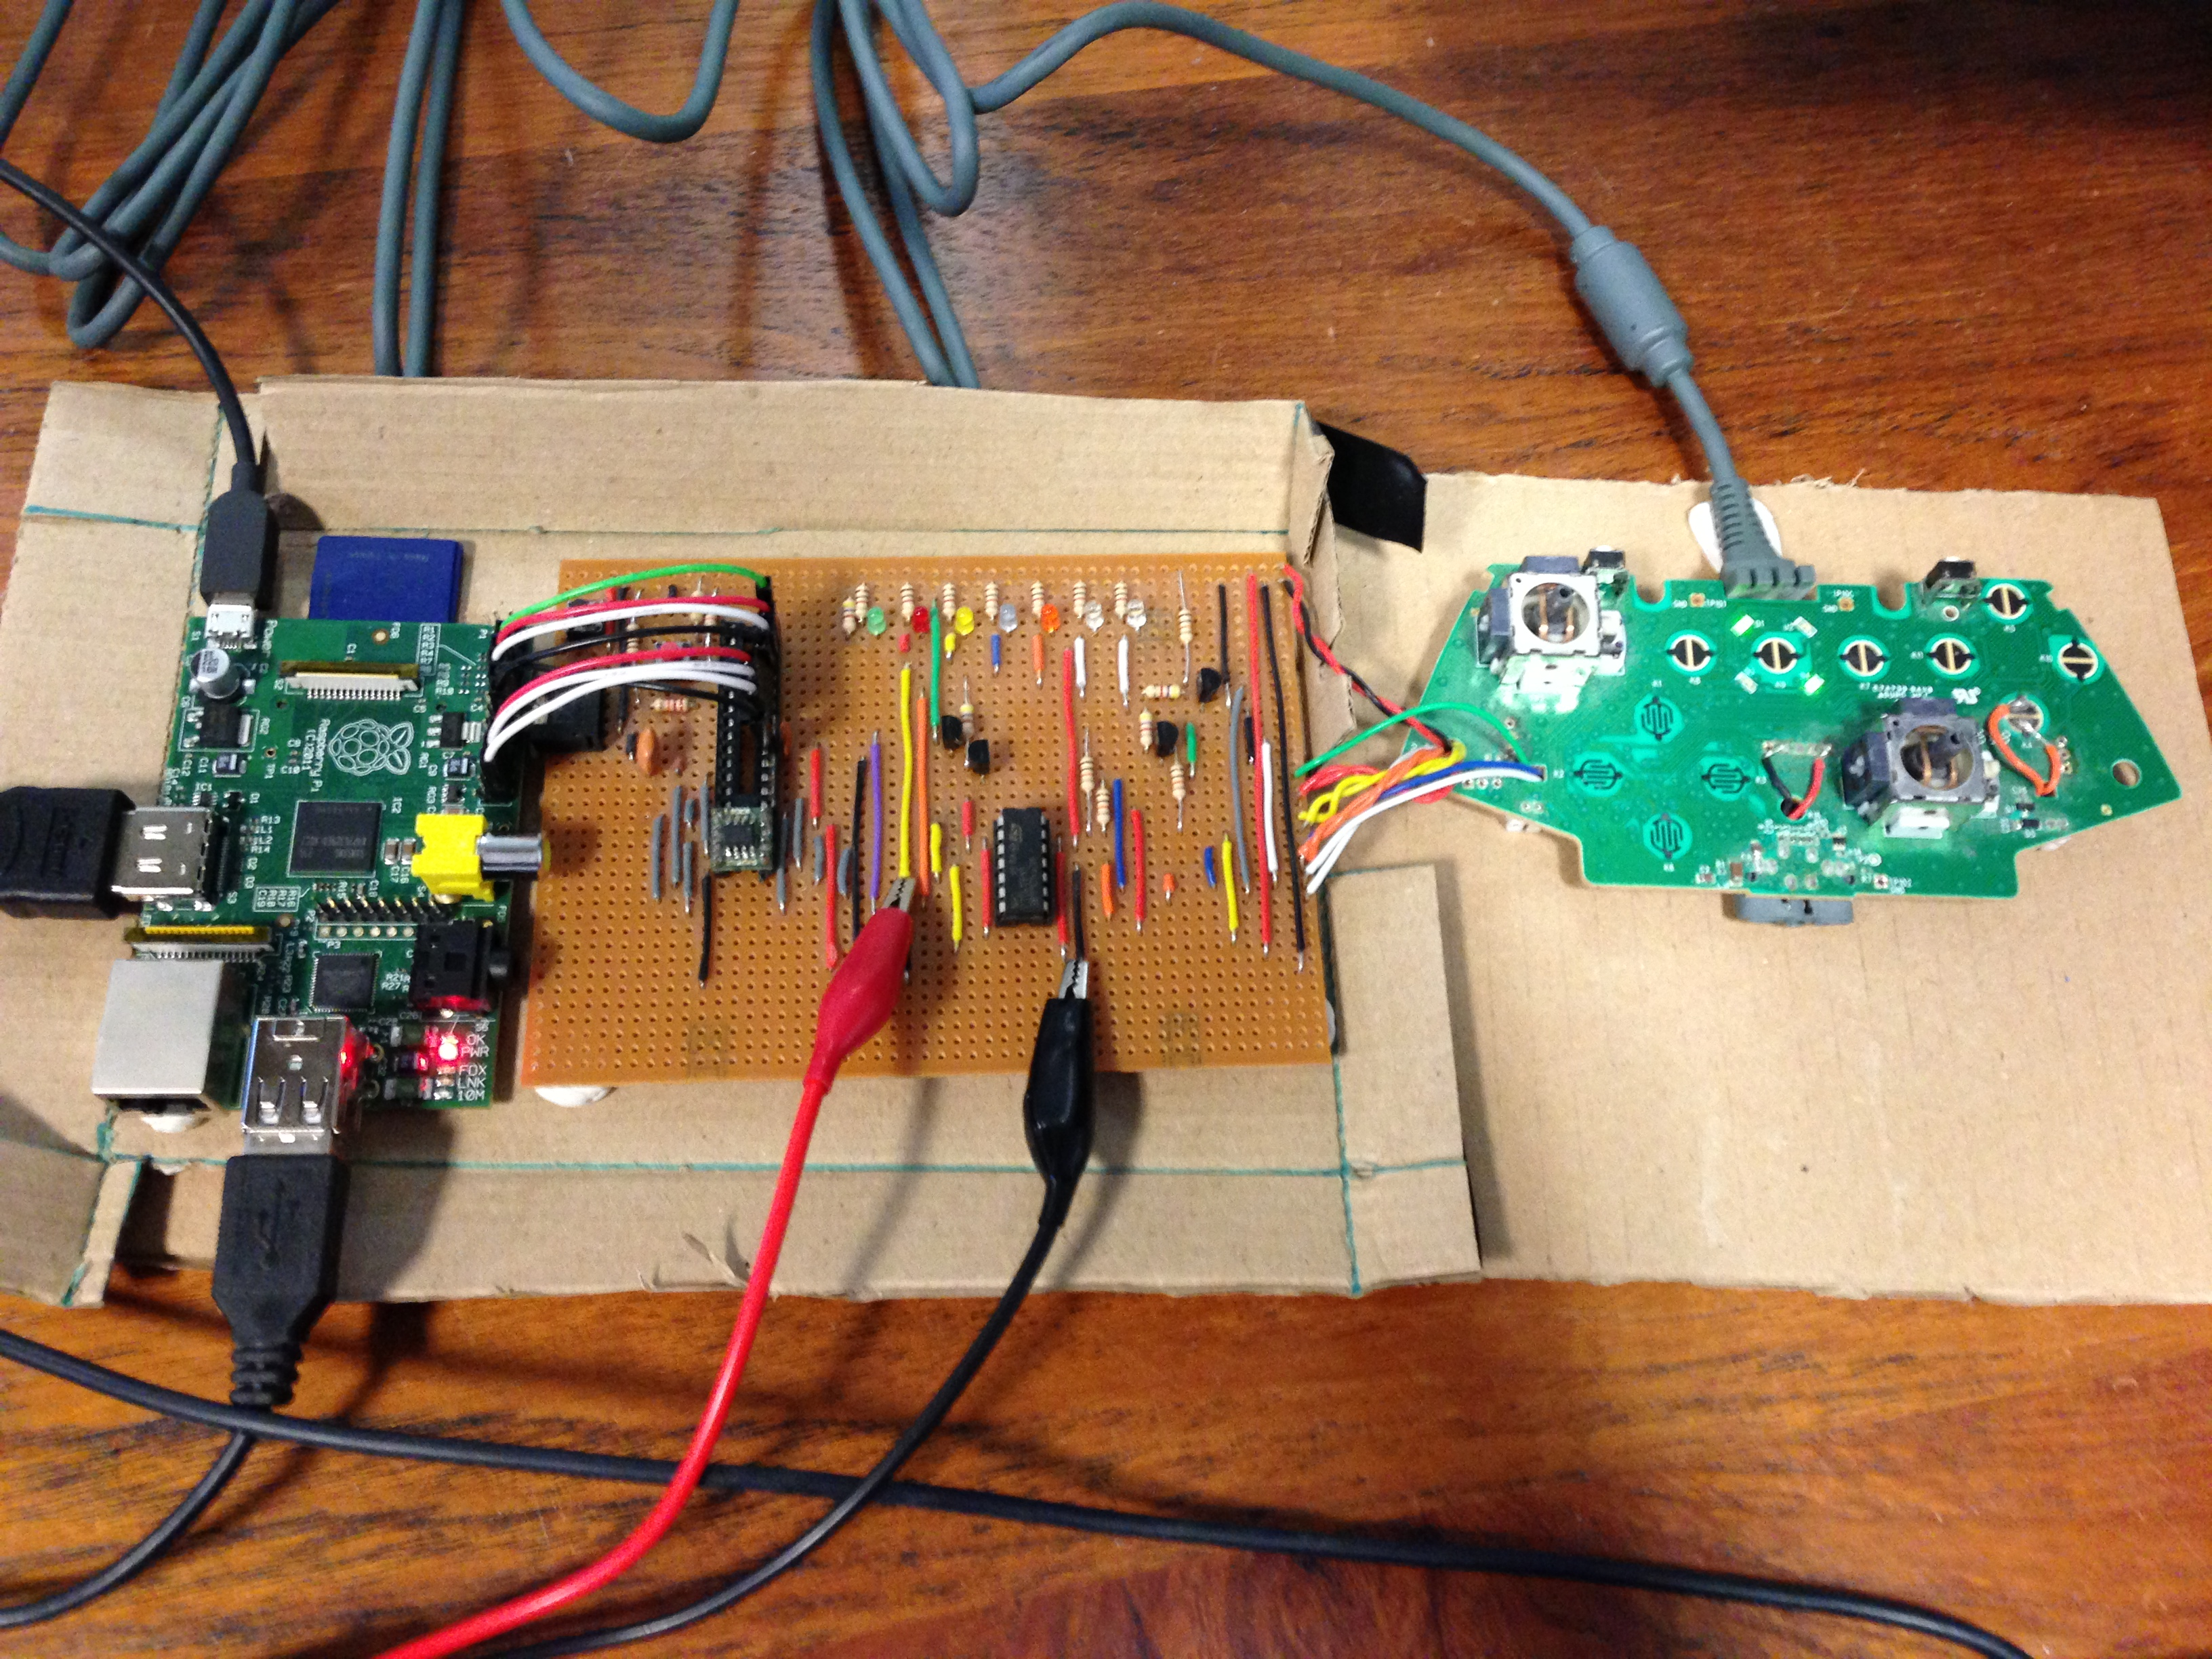
\includegraphics[width=0.3\textwidth]{IMG_9457.JPG}
    \caption{Interfacing circuit}
  \end{center}
  \vspace{-10pt}
\end{wrapfigure}

We decided to do this by writing a MAlice program to play \emph{Guitar Hero 3} on an Xbox 360 console. We built a simple electronic circuit with some NPN transistors and a 4066 logic chip to interface with a wired USB Xbox 360 controller. By connecting this circuit to the Raspberry Pi's GPIO pins (all set to outputs), we had the Pi playing notes in the game. All we had to do then was write a MAlice program to play a song, which we produced automatically using the note data from the game. In order to do this, we had to introduce one further new MAlice command:

\begin{verbatim}
    Alice slept for 16 milliseconds. ### sleep for 16ms

\end{verbatim}

Our first attempt at MAlice playing \emph{Guitar Hero} resulted in the timing of the notes being slightly off. To investigate this, we borrowed a digital oscilloscope from Imperial College Robotics Society to work out what was going on. It transpired that our program was in fact accurate to the millisecond, and that our problem lied elsewhere.

We soon patched up the problem, and had our MAlice program scoring 100\% on the most difficult song in the game, at highest difficulty.

A (poor quality) video of our MAlice program playing \emph{Guitar Hero} can be viewed at\\
\url{https://vimeo.com/55601178}

\end{document}
